\documentclass[UTF8,adobefonts]{ctexart}
\usepackage{graphicx}
\usepackage{enumitem}
\usepackage{amsmath}
\usepackage{amsthm}
\usepackage{hyperref}
\newtheorem{theorem}{定理}
\newtheorem*{theorem1a}{定理 1-A}
\newtheorem*{corollary}{推论}
\newcommand{\boldPhi}{\boldsymbol{\Phi}}
\newcommand{\boldDelta}{\boldsymbol{\Delta}}
\begin{document}
\title{处理线性滤波以及预测问题的一种新途径}
\author{R. E. Kalman}
\date{}
\maketitle
\section{引言}
通讯与控制中的理论与实际问题中有很重要的一类具有统计性质。这样的问题有:(1)、随机信号的预测;(2)、从随机噪声中分离随机信号;(3)、在有噪声的情况下探测已知形式的信号(脉冲、正弦波)。

在Wiener开拓性的工作中,他证明\cite{rf1}从问题(1)和问题(2)可导出所谓Wiener-Hopf积分方程;他同样给出了解决具有实际重要意义的特殊情况——定态统计和有理数频谱——之积分方程的方法(频谱因式分解)。

在Wiener的基础性工作之后出现了许多延伸和推广。Zadeh与Ragazzini给出了有限存储器情况的解\cite{rf2}。Bode和Shannon\cite{rf3}同时独立的给出上述情况的解,并且给出了简化的求解方法。Booton讨论了非定态统计Wiener-Hopf方程\cite{rf4}。这些结果现在都写入了标准教科书中\cite{rf5,rf6}。最近Darlington\cite{rf7}沿着这些主线给出了一种稍微有些不同的方法。对抽样信号的延伸,参见Franklin\cite{rf8}和Lees\cite{rf9}的工作。基于Wiener-Hopf方程(同样应用于非定态问题,尽管前述方法一般并非如此)特征函数的方法由Davis\cite{rf10}开创并被许多其他人应用,例如Shinbrot\cite{rf11}, Blum\cite{rf12}, Pugachev\cite{rf13}, Solodovnikov\cite{rf14}.

在所有这些工作中,目标都是获取一个线性动力系统的明确说明(Wiener滤波器),由此可以完成预测、分离或者探测随机信号。

现有求解Wiener问题的方法受制于若干限制,这样就使得它们的实际用处收到削弱:
\begin{enumerate}
\item 最佳的滤波器由其脉冲响应具体指定。由这些数据合成滤波器并非易事。
\item 数值确定最佳的脉冲响应往往十分复杂并且不很适合机器计算。这种情况随着问题复杂度的增加而迅速变得更为糟糕。
\item 重要的推广(如增长存储器滤波器、非定态预测)需要新的推导过程,经常给非专业人士带来相当大的困难。
\item 这些推导过程的数学部分并不透明。基本假设及其后果趋于模糊。
\end{enumerate}

本文回避上述困难,提出看待这些问题的整个集合的新方式。以下是本文的亮点:
\begin{enumerate}[resume]
\item \emph{最佳估计和正交投影。}Wiener问题是以条件分布与期望的观点处理的。这样,Wiener理论的基本事实可以迅速获取;结果的范围以及基本假设可以清楚的显现出来。可以看到所有的统计计算以及结果都基于一阶和二阶平均;不需要其他的统计数据。这样一来困难(4)便被排除。这种方法在概率论中为人们所熟知(见Doob\cite{rf15}第148至155页以及Lo\`eve\cite{rf16}第455至464页),但在工程上还没有大量的应用。
\item \emph{随机过程模型。} 继前人之后,尤其是Bode与Shannon\cite{rf3}, 任意随机信号可以被表示(直到二阶平均统计性质)为线性动力系统受独立或不相关随机信号(“白噪声”)激励后的输出。这是工程上应用Wiener理论的标准手法\cite{rf2,rf3,rf4,rf5,rf6,rf7}。这里用到的方法与传统方法相比只在线性动力系统的描述方法上不同。我们将强调\emph{状态}以及\emph{状态过渡};换言之,线性系统将以一阶差分(或微分)方程组来刻画。为了利用(5)中提到的简化,这种观点是自然的,也是必要的。
\item \emph{求解Wiener问题。}使用状态——过渡方法,单独一次推导即覆盖多种问题:增长与有限存储器滤波器、定态与非定态统计等等;(3)中的困难消失了。正确猜测出估计问题的“状态”后,接下来就是最佳估计误差协方差矩阵的非线性差分(或微分)方程。这个方程与Wiener-Hopf方程有些相似。对方称的求解开始于观测开始的$t_0$时刻;随后每个时刻$t$方程的解都代表给定区间$(t_0, t)$上观测的最佳预测误差协方差。从$t$时刻的协方差矩阵我们立刻可以获得刻画最佳线性滤波器的系数,而无需进一步的计算。
\item \emph{对偶问题。}对Wiener问题的新的公式化使其接触到基于“状态”观点的成长中的控制系统新理论\cite{rf17,rf18,rf19,rf20,rf21,rf22,rf23,rf24}。令人惊讶的是,Wiener问题是无噪声最佳调整器问题的对偶,而此问题已经被本文的作者利用状态——过渡方法解决\cite{rf18,rf23,rf24}。两个问题的数学背景完全一致——这一点一直以来都被人们所怀疑,但直到现在两者的类比才被明确指出。
\item \emph{应用。}新方法的威力在理论调研与复杂实际问题的数值解答中大多显而易见。在后面的案例中,最好借助机器计算。这种类型的例子将在后面讨论。为了给应用提供一些感觉,包含了两个非定态预测的标准例子;在这些例子中,(7)中提到的非线性差分方程甚至可以得到近似形式的解。
\end{enumerate}

为了参考方便,主要结果都用定理的形式显示。只有定理3和定理4是原创的。下一个章节以及附录主要服务于用适用于当前目的的形式来回顾人们熟知的资料。

\section{符号约定}
贯穿本文,我们主要与\emph{离散}(或者\emph{抽样})动力系统打交道;换句话说,信号将在等间距的时刻(\emph{抽样瞬间})被观测到。选择合适的时间尺度,相邻两次抽样瞬间的时间间隔常数(\emph{抽样周期})可以被选择为单位时间。如此一来,表示时间的变量如$t$, $t_0$, $\tau$, $T$等将一直是整数。对离散动力系统施加这样的约束条件并不是必需的(至少从工程的角度来看是这样);使用这样的离散性,我们可以保有严密的、基础的数学。矢量将用小写粗体字母如$\mathbf{a}, \mathbf{b}, \dotsc, \mathbf{x}, \mathbf{y}, \dotsc$表示。矢量,或者更精确的说,$n$维矢量是$n$个数$x_1, \dotsc, x_n$的集合;$x_i$是矢量$\mathbf{x}$的\emph{坐标}或\emph{分量}。

矩阵将使用大写粗体字母$\mathbf{A}, \mathbf{B}, \mathbf{Q}, \boldsymbol{\Phi}, \boldsymbol{\Psi}, \dotsc$表示;它们是元素$a_{ij}$, $b_{ij}$, $q_{ij}$, $\dotsc$的$m \times n$维数列。矩阵的\emph{转置}(交换行与列)用一撇来表示。使用公式时,为求方便,视矩阵为只有一列元素的矩阵。

使用传统的矩阵乘法定义,我们将两个$n$维矢量$\mathbf{x}, \mathbf{y}$的\emph{标量积}写成
\begin{equation*}
\mathbf{x'}\mathbf{y}=\sum^n_{i=1}x_i y_i=\mathbf{y'}\mathbf{x}
\end{equation*}
标量积显然是标量,也就是说并非矢量。类似的,关于$n \times n$维矩阵$\mathbf{Q}$的二次型是,
\begin{equation*}
\mathbf{x'Qy}=\sum^n_{i,j=1}x_i q_{ij} x_j
\end{equation*}
我们定义表达式$\mathbf{xy'}$(式中$\mathbf{x'}$是$m$维矢量,$\mathbf{y}$是$n$维矢量)为$m \times n$维矩阵,矩阵元为$x_i y_j$.

我们将随机矢量$\mathbf{x}$的期望值记为$E(\mathbf{x})=E\mathbf{x}$(见附录)。为方便起见,通常省略$E$后面的括号。因为常数与$E$算符对易,故这种省略在简单情况中并不会引起混淆。从而,$E\mathbf{xy'}$是矩阵元为$E(x_i y_j
)$的矩阵;$E\mathbf{x}E\mathbf{y}$是以$E(x_i)E(y_j)$为矩阵元的矩阵。

为方便参考,下面给出基本符号表:
\begin{table}[htbp]
\centering
\begin{tabular}{rl}
    \multicolumn{2}{l}{\heiti{最佳估计}}\\
    $t$ & 时间,当前时间。\\
    $t_0$ & 观测开始时刻。\\
    $x_1(t), x_2(t)$ & 基本随机变量。\\
    $y(t)$ & 观测到的随机变量。\\
    $x_1^\ast(t_1 \vert t)$ & 给定$y(t_0),\dotsc, y(t)$之后对$x_1(t_1)$的最佳估计。\\
    $L$ & 损耗函数(是其自变量的非随机函数)。\\
    $\epsilon$ & 估计误差(随机变量)。\\
    \multicolumn{2}{l}{\heiti{正交投影}}\\
    $\mathbf{\mathcal{Y}}(t)$ & 随机变量$y(t_0), \dotsc, y(t)$生成的线性流形。\\
    $\bar{x}(t_1 \vert t)$ & $x(t_1)$在$\mathbf{\mathcal{Y}}(t)$上的正交投影。\\
    $\tilde{x}(t_1 \vert t)$ & $x(t_1)$正交于$\mathbf{\mathcal{Y}}(t)$的分量。\\
    \multicolumn{2}{l}{\heiti{随机过程模型}}\\
    $\boldsymbol{\Phi}(t+1 ; t)$ & 过渡矩阵。\\
    $\mathbf{Q}(t)$ & 随机激励的协方差。\\
    \multicolumn{2}{l}{\heiti{求解Wiener问题}}\\
    $\mathbf{x}(t)$ & 基本随机变量。\\
    $\mathbf{y}(t)$ & 观测到的随机变量。\\
    $\mathbf{\mathcal{Y}}(t)$ & 由$\mathbf{y}(t_0), \dotsc, \mathbf{y}(t)$生成的线性流形。\\
    $\mathbf{\mathcal{Z}}(t)$ & 由$\tilde{\mathbf{y}}(t \vert t-1)$生成的线性流形。\\
    $\mathbf{x}^\ast(t_1 \vert t)$ & 给定$\mathbf{\mathcal{Y}}(t)$之后对$\mathbf{x}(t_1)$的最佳估计。\\
    $\tilde{\mathbf{x}}(t_1 \vert t)$ & 给定$\mathbf{\mathcal{Y}}(t)$之后对$\mathbf{x}(t_1)$最佳估计的误差。
\end{tabular}
\end{table}

\section{最佳估计}
为具体描述将要研究问题的类型,需考虑以下情况。已知信号$x_1(t)$和噪声$x_2(t)$. 只能观察到和$y(t)=x_1(t)+x_2(t)$. 假定我们已经观测并确切的知道$y(t_0), \dotsc, y(t)$的值,关于$t=t_1$($t_1$可能小于、等于或者大于$t$)处的值(非观测量)我们可以从已知信息中推断出什么?如果$t_1 < t$, 这是\emph{数据平滑(插值)}问题。如果$t_1 = t$, 这称为\emph{滤波}。如果$t_1 > t$ ,称为\emph{预测}问题。既然我们有足够一般性的方法来处理以上以及类似的问题,以下我们将使用共同的术语\emph{估计}。

正如Wiener指出\cite{rf1}的那样,估计问题的天然背景属于概率论和统计学的范畴。因此信号、噪声以及它们的和都是随机变量,进而它们可被视为随机过程。从随机过程的概率论描述中我们可以确定特定信号或者噪声抽样发生的概率。对于随机变量$y(t)$的任意给定的测量值$\eta(t_0),\dotsc, \eta(t)$原则上也可以确定随机变量$x_1(t_1)$于同一时刻取不同值$\xi_1(t)$的概率。这就是条件概率分布函数
\begin{equation}
\label{eq1}
Pr[x_1(t_1) \le \xi_1 \vert y(t_0)=\eta(t_0),\dotsc, y(t)=\eta(t)]=F(\xi_1)
\end{equation}
显然,$F(\xi_1)$代表了随机变量$y(t_0), \dotsc, y(t)$测量结果传递的关于随机变量$x_1(t_1)$所有信息。随机变量$x_1(t_1)$的任何统计估计都是上述分布的某种函数,因而是随机变量$y(t_0), \dotsc, y(t)$的(非随机)函数。该统计估计记为$X_1(t_1 \vert t)$, 如果观测到的随机变量集合或者待估计时间在上下文中是明确的,也可记为$X_1(t_1)$或者$X_1$.

假定$X_1$以随机变量$y(t_0), \dotsc, y(t)$的固定函数的形式给出。那么$X_1$本身就是一个随机变量,只要$y(t_0), \dotsc, y(t)$的实际值已知,即可知$X_1$的实际值。一般来说,$X_1(t_1)$的实际值与$x_1(t_1)$的(未知)实际值是不同的。为了取得确定$X_1$的合理方法,自然要为不正确的估计指定\emph{罚函数}或\emph{损耗函数}。确切的说,损耗函数应当(1)非负,(2)是\emph{估计误差}$\epsilon=x_1(t_1)-X_1(t_1)$的单调不递减函数。故此,定义损耗函数
\begin{equation*}
L(0)=0
\end{equation*}
\begin{equation}
\label{eq2}
L(\epsilon_2) \le L(\epsilon_1) \le 0 \text{ when } \epsilon_2 \le \epsilon_1 \le 0
\end{equation}
\begin{equation*}
L(\epsilon)=L(-\epsilon) 
\end{equation*}
常见的损耗函数有:$L(\epsilon)=a \epsilon ^2,a \epsilon ^4,a \vert \epsilon \vert,a[1-exp(-\epsilon^2)]$等等,其中$a$是大于零的常数。

一种(但并非唯一的)自然而然的选择随机变量$X_1$的方法是令选取的值最小化损耗或风险的平均值
\begin{equation}
\label{eq3}
E\{L[x_1(t_1)-X_1(t_1)]\}=E[E\{L[x(t_1)-X_1(t_1)] \vert y(t_0), \dotsc, y(t)\}]
\end{equation}
既然式\ref{eq3}右边第一个期望值不依赖于$X_1$的选择,而是由$y(t_0), \dotsc, y(t)$唯一决定,所以最小化ref{eq3}等价于最小化
\begin{equation}
\label{eq4}
E\{L[x_1(t_1)-X_1(t_1)] \vert y(t_0), \dotsc, y(t)\}
\end{equation}
在少量附加的假设之下,最佳估计就可以用简单的方法刻画出来。
\begin{theorem}
\label{th1}
假定$L$如式\ref{eq2}且由式\ref{eq1}定义的条件分布函数$F(\xi)$:
\begin{itemize}
\item[A] 关于均值$\bar{\xi}$对称:
    \begin{equation*}
    F(\xi-\bar{\xi})=1-F(\bar{\xi}-xi)
    \end{equation*}
\item[B] 对$\xi \le \bar{\xi}$是凸的:
    \begin{multline*}
    F(\lambda\xi_1+(1-\lambda)\xi_2) \le \lambda F(\xi_1)+(1-\lambda)F(\xi_2)\\
    \text{for all }\xi_1,\xi_2 \le \bar{\xi} \text{ and } 0 \le \lambda \le 1
    \end{multline*}
\end{itemize}
则最小化损耗(式\ref{eq3})的随机变量$x^{\ast}_1(t_1 \vert t)$是条件期望
\begin{equation}
\label{eq5}
x^{\ast}_1(t_1 \vert t)=E[x_1(t_1) \vert y(t_0),\dotsc,y(t)]
\end{equation}
\end{theorem}
{\heiti{证明:}}
正如Sherman最近所指出\cite{rf25}的,该定理是概率论中一个著名引理的直接结论。

\begin{corollary}
如果随机过程${x_1(t),x_2(t)}$和${y(t)}$是高斯的,则定理\ref{th1}成立。
\end{corollary}
{\heiti{证明:}}
由定理\ref{th5}(见附录),高斯随机过程的条件概率仍然是高斯的。因而总是满足定理\ref{th1}的要求。

在控制系统的文献中,上面的定理以某种程度上更为受限而换言之也更为一般的形式出现:
\begin{theorem1a}
\label{th1a}
如果$L(\epsilon)=\epsilon^2$, 那么无需假设A和B定理\ref{th1}即成立。
\end{theorem1a}
{\heiti{证明:}}
展开条件期望(式\ref{eq4}):
\begin{equation*}
E[x_1^2(t_1) \vert y(t_0),\dotsc,y(t)]-2X_1(t_1)E[x_1(t_1) \vert y(t_0),\dotsc,y(t)]+X_1^2(t_1)
\end{equation*}
然后对$X_1(t_1)$求导。这并非严密的论证;若求简单严密的论证可参考Doob专著的第77至78页。

{\heiti{评论。}}(一)、就作者所知,人们并不知道条件分布函数满足定理\ref{th1}要求的随机过程${x_1(t),x_2(t)}$属于何种最为一般的类型。

(二)、除了Sherman的记录,定理\ref{th1}似乎从来没有在控制系统的文献中明确出现过。事实上,一般类型(如式\ref{eq2})的损耗函数在数学上无法方便的处理,对这种影响的陈述随处可见。

(三)、后文中,我们将主要应付矢量值随机变量。相应的,估计问题表述为:给定矢量值随机过程${\mathbf{x}(t)}$和观测随机变量$\mathbf{y}(t_0),\dotsc,\mathbf{y}(t)$, 其中$\mathbf{y}(t)=\mathbf{Mx}(t)$($\mathbf{M}$是奇异矩阵;换句话说,并非$\mathbf{x}(t)$的所有坐标都能被观测到),试求可以最小化损耗期望$E[L(\Vert\mathbf{x}(t_1)-\mathbf{X}(t_1)\Vert)]$的估计$\mathbf{X}(t_1)$, $\Vert\text{ }\Vert$是矢量的范数。

定理\ref{th1}在矢量情况下依然成立,只要矢量$\mathbf{x}(t_1)$的$n$个分量的条件分布函数
\begin{equation*}
Pr[x_1(t_1) \le \xi_1,\dotsc,x_n(t_1) \le \xi_n \vert \mathbf{y}(t_0),\dotsc,\mathbf{y}(t)]=F(\xi_1,\dotsc,\xi_n)
\end{equation*}
关于$n$个变量$\xi_1-\bar{\xi}_1,\dotsc,\xi_n-\bar{\xi}_n$对称且在所有这些变量取负值的区域是凸的。


\section{正交投影}
一般来说,作为观测变量的函数准确计算最佳估计是不可能的。但这里有个重要的例外:过程${x_1(t)}$和${x_2(t)}$是高斯的。

另一方面,如果令损耗函数$L(\epsilon)=\epsilon^2$且令估计是观测随机变量的线性函数,我们将得到与高斯情形相同的最佳估计,而高斯情形则无需线性性质以及二次型损耗函数的假设。这证明非线性估计仅在以下情况能得到优于线性估计的结果:(一)、随机过程不是高斯的(依定理\ref{th5}中C的观点),且(二)、要至少考虑三阶的概率分布函数。

在上面提到的特殊情况中,显式求解估计问题在几何图像的帮助下大致上可以容易理解一些。这正是本部分的主旨。

考虑(实值)随机变量$y(t_0),\dotsc,y(t)$. 系数为实数的这些随机变量的所有线性组合的集合
\begin{equation}
\label{eq6}
\sum^t_{i=t_0}a_i y(i)
\end{equation}
构成一个矢量空间(线性流形),记为$\mathbf{\mathcal{Y}}(t)$. 我们将所有形如式\ref{eq6}的表达式抽象的视为$\mathbf{\mathcal{Y}}(t)$上的“点”或“矢量”。当然,此处使用的“矢量”当不与随机矢量中的“矢量”或者其它地方的“矢量”相混淆。由于我们并不想限定$t$的值(可能的观测的总数),故$\mathbf{\mathcal{Y}}(t)$应该被视为所有可能的观测空间的有限维子空间。

任意给定$\mathbf{\mathcal{Y}}(t)$中的两个矢量$u\text{, }v$(即可由式\ref{eq6}表达的随机变量),如果$Euv=0$我们就说$u\text{, }v$是正交的。使用Schmidt正交化过程,正如Doob\cite{rf15}(第151页)或Lo\`eve\cite{rf16}(第459页)借助实例描绘的,很容易就可以找出$\mathbf{\mathcal{Y}}(t)$的一组正交基,亦即,$\mathbf{\mathcal{Y}}(t)$的一组正交矢量$e_{t_0},\dotsc,e_t$, 使用这组矢量,$\mathbf{\mathcal{Y}}(t)$中的任意矢量都可以被唯一的表示为$e_{t_0},\dotsc,e_t$的线性组合,且
\begin{equation}
\label{eq7}
\left.\begin{aligned}
Ee_ie_j=\delta_{ij}&=1 \text{ 如果 } i = j\\
&=0 \text{ 如果 } i \ne j
\end{aligned}\right\}
\qquad (i,j=t_0,\dotsc,t)
\end{equation}
故$\mathbf{\mathcal{Y}}(t)$中的任意矢量可写成
\begin{equation*}
\bar{x}=\sum^t_{i=t_0}a_ie_i
\end{equation*}
系数$a_i$也可借由\ref{eq7}立刻得出
\begin{equation}
\label{eq8}
E\bar{x}e_j=E[\sum^t_{i=t_0}a_ie_i]e_j=\sum^t_{i=t_0}a_iEe_ie_j=\sum^t_{i=t_0}\delta_{ij}=a_j
\end{equation}

进一步的,所有随机变量$x$(并不一定是$\mathbf{\mathcal{Y}}(t)$中的)可以唯一的被分解成两部分:一部分为$\bar{x}$在$\mathbf{\mathcal{Y}}(t)$中,另一部分同$\mathbf{\mathcal{Y}}(t)$正交(即同$\mathbf{\mathcal{Y}}(t)$中所有矢量都正交)。事实上,我们可以将其写为
\begin{equation}
\label{eq9}
x=\bar{x}+\tilde{x}=\sum^t_{i=t_0}(Exe_i)e_i+\tilde{x}
\end{equation}
故$\bar{x}$可以由式\ref{eq9}唯一确定,且显然是$\mathbf{\mathcal{Y}}(t)$中的矢量。这样$\tilde{x}$也被唯一的确定了;接下来检验其是否与$\mathbf{\mathcal{Y}}(t)$正交:
\begin{equation*}
E\tilde{x}e_i=E(x-\bar{x})e_i=Exe_i-E\bar{x}e_i
\end{equation*}

$\bar{x}$关于基$e_{t_0},\dotsc,e_t$的坐标或者如式\ref{eq8}以$E\bar{x}e_i$的形式给出,或者如式\ref{eq9}以$Exe_i$的形式给出。既然坐标是唯一的,故$Exe_i=E\bar{x}e_i\text{ }(i=t_0,\dotsc,t)$;因此$E\tilde{x}e_i=0$, $\tilde{x}$与每个基矢量$e_j$都正交;也就是说与$\mathbf{\mathcal{Y}}(t)$正交。我们称$\tilde{x}$为$x$在$\mathbf{\mathcal{Y}}(t)$上的\emph{正交投影}。

这里还有另外一种表征正交投影的方式:$\bar{x}$是$\mathbf{\mathcal{Y}}(t)$上最小化二次型损耗函数的矢量(即随机变量$y(t_0),\dotsc,y(t)$的线性组合)。事实上,如果$\bar{w}$是$\mathbf{\mathcal{Y}}(t)$上的任意另一矢量,有
\begin{equation*}
E(x-\bar{w})^2=E(\tilde{x}+\bar{x}-\bar{w})^2=E[(x-\bar{x})+(\bar{x}-\bar{w})]^2
\end{equation*}

既然$\tilde{x}$与$\mathbf{\mathcal{Y}}(t)$上的所有矢量,特别的,与$\bar{x}-\bar{w}$正交,有
\begin{equation}
\label{eq10}
E(x-\bar{w})^2=E(x-\bar{x})^2+E(\bar{x}-\bar{w})^2 \ge E(x-\bar{x})^2
\end{equation}
恰好证明,如果$\bar{w}$也最小化二次型损耗函数,则必有$E(\bar{x}-\bar{w})^2=0$, 即,随机变量$\bar{x}$和$\bar{w}$相等(除非对于概率为零的一组事件)。

以上结果摘要如下:
\begin{theorem}
\label{th2}
令$\{x(t)\},\{y(t)\}$为零均值的随机过程(即,对于一切$t$均有$Ex(t)=Ey(t)=0$)。观测$y(t_0),\dotsc,y(t)$.

如果有
\begin{itemize}
\item[A] 随机过程$\{x(t)\},\{y(t)\}$是高斯的;或者
\item[B] 将最佳估计限定为观测随机变量的线性函数且$L(\epsilon)=\epsilon^2$;
\end{itemize}
那么
\begin{multline}
\label{eq11}
x^\ast (t_1 \vert t)=\text{给定}y(t_0),\dotsc,y(t)\text{对}x(t_1)\text{的最佳估计}\\
=x(t_1)\text{在}\mathbf{\mathcal{Y}}(t)\text{上的正交投影}。
\end{multline}
\end{theorem}

以上结果为人们所熟知,尽管这在控制系统文献中并不容易获取。见Doob\cite{rf15}第75至78页,或着Pugachev\cite{rf26}。有时为求方便,将正交投影记为
\begin{equation*}
\bar{x}(t_1 \vert t) \equiv x^\ast (t_1 \vert t)=\hat{E}[x(t_1) \vert \mathbf{\mathcal{Y}}(t)]
\end{equation*}
使用记号$\hat{E}$的目的是:如果讨论的随机过程是高斯的,则正交投影盒条件期望事实上是一样的。

{\heiti{证明:}}
\begin{itemize}
\item[A] 关于式\ref{eq10}评论的直接结果。
\item[B] 既然$x(t),y(t)$都是零均值的随机变量,从式\ref{eq9}可知,$x(t_1)$关于$\mathbf{\mathcal{Y}}(t)$的正交部分$\tilde{x}(t_1 \vert t)$也是零均值的随机变量。零均值随机变量是不相关的;如果同时他们也是高斯的(由于定理\ref{th5}B部分),则他们是独立的。所以
\begin{equation*}
\begin{split}
0=E\tilde{x}(t_1 \vert t)&=E[\tilde{x}(t_1 \vert t)\vert y(t_0),\dotsc,y(t)]\\
&=E[x(t_1) - \bar{x}(t_1 \vert t)\vert y(t_0),\dotsc,y(t)]\\
&=E[x(t_1)\vert y(t_0),\dotsc,y(t)]-\bar{x}(t_1 \vert t)=0
\end{split}
\end{equation*}
\end{itemize}

{\heiti{评论。}}
(四)、$t \to \infty$时本部分内容的严格公式化需要希尔伯特空间的一些基本概念。见Doob\cite{rf15}与Lo\`eve\cite{rf16}。

(五)、定理\ref{th2}的物理学阐述大体上。如果我们不担心高斯性质的假设,A部分证明正交投影是所有合理损耗函数的最佳估计。如果我们确实担心高斯性质的假设,甚至我们只考虑线性估计,对于多数合理的损耗函数而言,正交投影都不是最佳估计。由于事实上一个有物理来源的随机过程在多大程度上是高斯的很难把握,定理\ref{th2}究竟具有很广泛的还是很有限的重要性也很难判断。

(六)、直接将定理\ref{th2}推广为矢量值随机变量的情况。事实上,定义$\mathbf{y}(t_0),\dotsc,\mathbf{y}(t)$生成的线性流形$\mathbf{\mathcal{Y}}(t)$为随机矢量$\mathbf{y}(t_0),\dotsc,\mathbf{y}(t)$中每一个的所有$m$个分量的所有线性组合
\begin{equation*}
\sum^t_{i=t_0}\sum^m_{j=1}a_{ij}y_j (i)
\end{equation*}
的集合。随后的部分可仿效前面的部分。

(七)、定理\ref{th2}有效的说明了,条件A或B下最佳估计是所有既往观测的线性组合。换言之,最佳估计可考虑成线性滤波器的输出,滤波器的输入是可观测随机变量实际发生的数值;定理\ref{th2}为计算最佳滤波器的脉冲响应提供了方法。正如前面指出的,对脉冲响应的认识并不是问题的完整的解;出于这个原因,不会给出计算脉冲响应的显式的公式。

\section{随机过程模型}
在同物理现象打交道时,仅仅给出经验性的描述是不够的,还必须对潜在的原因有一定了解。如果不能在某种意义上区分原因和影响,亦即,如果没有因果关系的假设,那么就几乎无法期待有用的结果。

通常人们都接受这样一个事实,即随机现象的主要宏观来源是独立的高斯过程。一个著名的例子是电阻中由热扰动造成的噪声电压。在大多数情况下,\emph{观测}到的随机现象不能通过独立的随机变量来描述。通常,不同时刻观测到的随机信号之间的统计依赖性(相关性)是由主要随机来源于观测者之间存在动力学系统来解释的。\emph{因此以时间为自变量的随机函数可以考虑为接受独立高斯随机过程激励的动力学系统的输出。}

高斯随机信号的一个重要属性是,当它们通过线性系统之后,它们仍然是高斯的(定理\ref{th5}的A部分)。假定有独立的、高斯的主要随机源,如果观测到的随机信号也是高斯的,我们即可假定观测者与主要源之间的动力学系统是\emph{线性的}。我们之所以必须接受这条结论,也是因为对观测到的随机信号的统计属性缺乏细致的了解:给定已知一阶、二阶平均的任意随机过程,我们可以找到具有相同属性的高斯随机过程(定理\ref{th5}的C部分)。因此,高斯分布和线性动力学性质是自然而然的、互为印证的假设,特别是当统计数据贫乏的时候。

一个动力学系统(线性的或非线性的)是如何被描述的?基本思想是\emph{状态}的概念。这意味着,直观的来说,一些定量的信息(数的集合、函数,等等)。如果要预测系统的未来行为,这些信息就是必须知道的有关系统过去行为的最少量数据。这样,动力学性质就用术语\emph{状态过渡}来描述,即,必须指出随着时间的流逝,状态是如何过渡成另一个状态的。

线性动力学系统一般可以用矢量微分方程
\begin{equation}
\label{eq12}
\left.\begin{aligned}
&d\mathbf{x}/dt=\mathbf{F}(t)\mathbf{x}+\mathbf{D}(t)\mathbf{u}(t)\\
\text{和}\qquad&\\
&\mathbf{y}(t)=\mathbf{M}(t)\mathbf{x}(t)
\end{aligned}\right\}
\end{equation}
表示,其中$\mathbf{x}$是$n$维矢量,系统的\emph{状态}($\mathbf{x}$的分量$x_i$称为系统的\emph{状态变量});$\mathbf{u}(t)$是$m$维($m \le n$)矢量,表示系统的\emph{输入};$\mathbf{F}(t)$和$\mathbf{D}(t)$分别是$n \times n$和$n \times m$维矩阵。如果$\mathbf{F}(t),\mathbf{D}(t),\mathbf{M}(t)$的所有系数都是常数,我们就说动力学系统(式\ref{eq12})是\emph{时不变}或\emph{定态}的。最后,$\mathbf{y}(t)$是$p$维矢量,表示系统的输出;$\mathbf{M}(t)$是$n \times p$维的矩阵;$p \le n$.

式\ref{eq12}的物理阐释已经在别的文献中详细讨论过\cite{rf18,rf20,rf23}。图\ref{fg1}或许有所帮助。这是一副矩阵框图(图中箭头指示信号流向)。图\ref{fg1}中的积分号事实上表示$n$个积分器,每个积分器的输出都是标量变量;$\mathbf{F}(t)$表明积分器的输出如何反馈到积分器的输入。故$f_{ij}(t)$是第$j$积分器的输出反馈到$i$积分器的输入的系数。将这种重视形式的方法与更为传统的线性系统分析方法联系起来并不困难。
\begin{figure}[htbp]
\centering
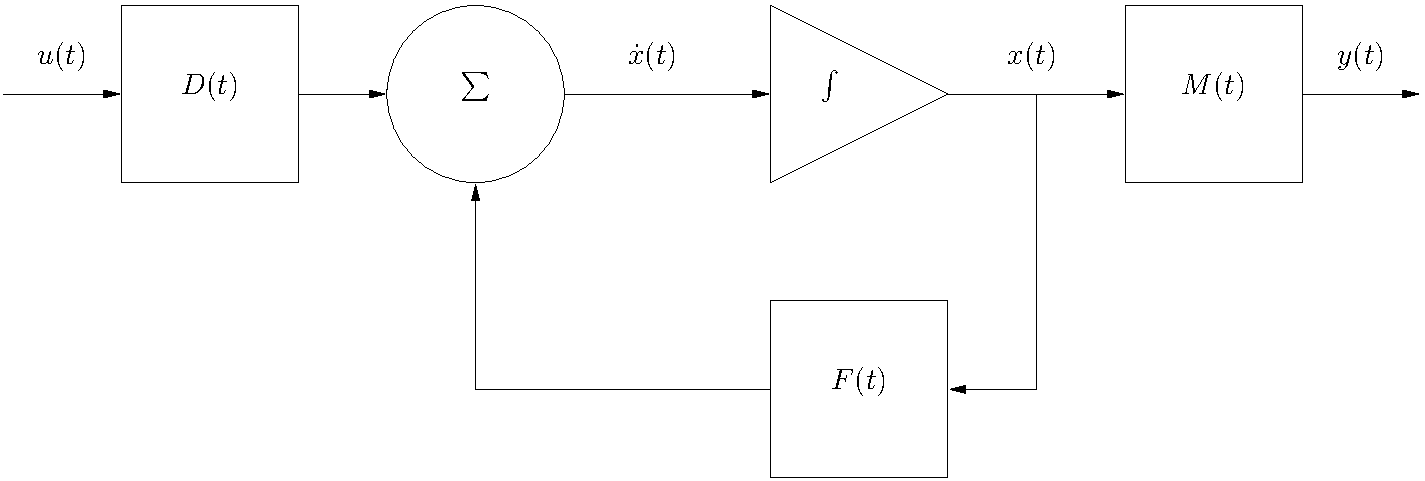
\includegraphics[width=0.5\paperwidth]{fig/fg1.pdf}
\caption{一般线性连续动力学系统的矩阵框图}
\label{fg1}
\end{figure}

如果我们假定如式\ref{eq12}的系统是定态的,$\mathbf{u}(t)$在每个抽样周期都不变,即
\begin{equation}
\label{eq13}
\mathbf{u}(t+\tau)=\mathbf{u}(t)\text{; }0 \le \tau < 1\text{, }t=0,1,\dotsc
\end{equation}
那么式\ref{eq12}立即可以变形成更方便的离散形式。
\begin{equation*}
\mathbf{x}(t+1)=\boldsymbol{\Phi}(1)\mathbf{x}(t)+\boldsymbol{\Delta}(1)\mathbf{u}(t)\text{; }t=0,1,\dotsc
\end{equation*}
其中\cite{rf18,rf20}
\begin{equation*}
\boldsymbol{\Phi}(1)=\exp\mathbf{F}=\sum^\infty_{i=0}\mathbf{F}^i/i!\text{ (}\mathbf{F}^0=\text{unit matrix}\text{)}
\end{equation*}
且
\begin{equation*}
\boldsymbol{\Delta}(1)=\left(\int^1_0 \exp\mathbf{F}\tau d \tau\right)\mathbf{D}
\end{equation*}
\begin{figure}[htbp]
\centering
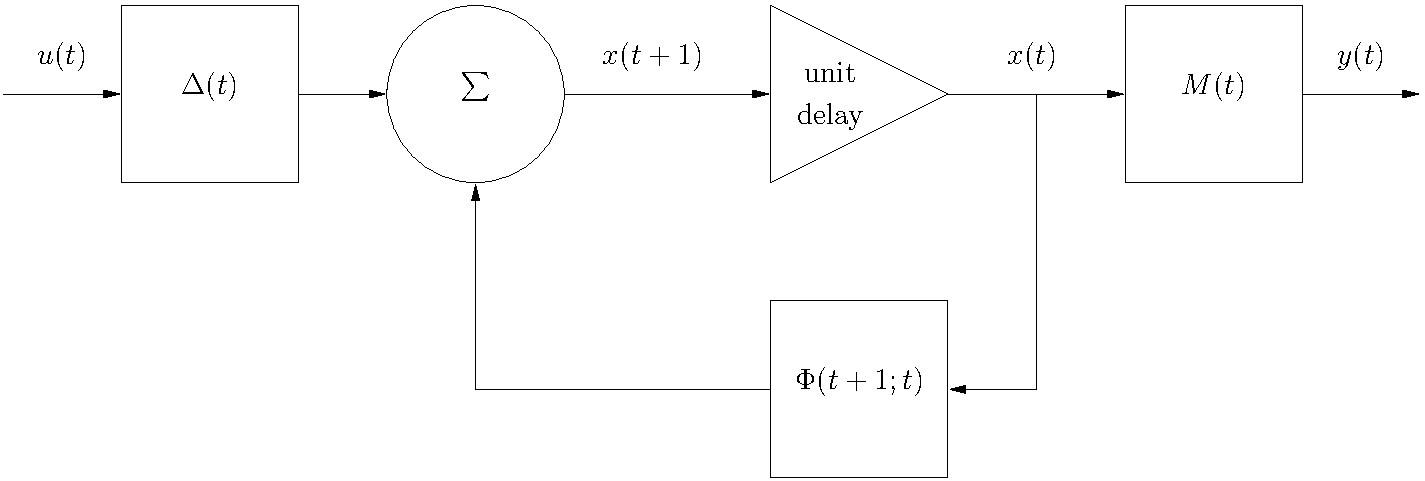
\includegraphics[width=0.5\paperwidth]{fig/fg2.pdf}
\caption{一般线性离散动力学系统的矩阵框图}
\label{fg2}
\end{figure}
见图\ref{fg2}。也可以通过拉普拉斯变换的方法\cite{rf18,rf20,rf22,rf24}将$\mathbf{F}\tau$表达成闭合的形式。如果$\mathbf{u}(t)$满足式\ref{eq13}但系统(式\ref{eq12}非定态,类似的
\begin{equation}
\label{eq14}
\left.\begin{aligned}
\mathbf{x}(t+1)&=\boldsymbol{\Phi}(t+1;t)+\boldsymbol{\Delta}(t)\mathbf{u}(t)\\
\mathbf{y}(t)&=\mathbf{M}(t)\mathbf{x}(t)
\end{aligned}\right\}
\qquad t=0,1,\dotsc
\end{equation}
但是显然现在无法用闭合形式表示$\boldsymbol{\Phi}(t+1;t),\boldsymbol{\Delta}(t)$. 形如式\ref{eq14}的方程也经常在研究复杂的抽样数据系统中遇到\cite{rf22}, 见图\ref{fg2}.

$\boldPhi(t+1;t)$是系统(如式\ref{eq12}或式\ref{eq14})的\emph{过渡矩阵}。记号$\boldPhi(t_2;t_1)$意味着从时刻$t_1$到时刻$t_2$的过渡。显然,$\boldPhi(t;t)=\mathbf{I}=\text{单位矩阵}$。如果系统(如式\ref{eq12})是定态的,那么$\boldPhi{t+1;t}=\boldPhi(t+1-t)=\boldPhi(1)=\text{常数}$。注意乘法规则:$\boldPhi(t;s)\boldPhi(s;r)=\boldPhi(t;r)$和倒数规则$\boldPhi^{-1}(t;s)=\boldPhi(s;t)$, 其中$t,s,r$都是整数。定态系统中,$\boldPhi(t;\tau)=\exp \mathbf{F}(t-\tau)$.

作为前面讨论的结果,我们将用
\begin{equation}
\label{eq15}
\mathbf{x}(t+1)=\boldPhi(t+1;t)\mathbf{x}(t)+\mathbf{u}(t)
\end{equation}
模型来代表随机性现象,其中$\{\mathbf{u}(t)\}$是矢量值独立高斯随机过程,均值为零,完全由
\begin{align*}
E\mathbf{u}(t)=0 \text{ 对于一切 } t;\\
E\mathbf{u}(t)\mathbf{u'}(s)=0 \text{ 如果 } t \ne s\\
E\mathbf{u}(t)\mathbf{u'}(t)=\mathbf{G}(t).
\end{align*}
描述(依照定理\ref{th5}C的观点)。当然(定理\ref{tm5}A),$\mathbf{x}(t)$也是零均值的高斯随机过程,但不是独立的。事实上,如果我们认为式\ref{eq15}处于稳定状态(假设是稳定系统),换句话说,如果我们忽略初始状态$\mathbf{x}(t_0)$, 那么
\begin{equation*}
\mathbf{x}(t)=\sum^{t-1}_{r=-\infty}\boldPhi(t;r+1)\mathbf{u}(r).
\end{equation*}
因此如果$t \ge s$有
\begin{equation*}
E\mathbf{x}(t)\mathbf{x'}(s)=\sum^{s-1}_{r=-\infty}\boldPhi(t;r+1)\mathbf{Q'}(r)\boldsymbol{\Phi'}(s;r+1).
\end{equation*}
那么如果我们设想一个线性动力学系统并且知道高斯随机激励的统计学属性,则可以简单的找到相应的高斯随机$\{\mathbf{x}(t)\}$过程属性。

但是在现实生活中,情况通常是相反的。给定协方差矩阵$E\mathbf{x}(t)\mathbf{x'}(s)$(或者甚至要试着从有限的统计数据中估计该矩阵)问题是得到式\ref{eq15}和$\mathbf{u}(t)$的统计学属性。这是实验与数据处理中很微妙且当前大部分悬而未决的问题。正如在大多数Wiener问题的工程学著作中那样,我们将发现从式\ref{eq15}的模型开始,将获得模型本身视为单独的问题是很方便的。的确,如果可能\emph{应该}将这两个问题联合优化;但是据作者所知并没有\emph{联合}优化问题方面的研究。

作为小结,有关随机过程的以下假设已经作出:

\emph{物理随机现象可认为是源于主要随机来源激励的动力学系统。假定主要随机来源为独立的高斯随机过程,均值为零;动力学系统是线性的。随机过程因此由模型(如式\ref{eq15})描述。不考虑如何从实验数据获取具体数值以表示模型。}

\section{求解Wiener问题}
让我们先来定义本文的主要问题。

{\heiti{问题一。}}\emph{考虑动力学模型}
\begin{equation}
\label{eq16}
\mathbf{x}(t+1)=\boldsymbol{\Phi}(t+1;t)\mathbf{x}(t)+\mathbf{u}(t)
\end{equation}
\begin{equation}
\label{eq17}
\mathbf{y}(t)=\mathbf{M}(t)\mathbf{x}(t)
\end{equation}
\emph{其中}$\mathbf{u}(t)$\emph{是一个}$n$\emph{维矢量零均值独立高斯随机过程,}$\mathbf{y}(t)$\emph{是一个}$p$\emph{维矢量(}$p \le n$\emph{),}$\boldsymbol{\Phi}(t+1;t)\text{, }\mathbf{M}(t)$\emph{分别是}$n \times n\text{, }p \times n$\emph{维矩阵,矩阵元是时间的非随机函数。}

\emph{给定}$\mathbf{y}(t_0)\text{, }\dotsc\text{, }\mathbf{y}(t)$\emph{的观测值},\emph{找到}$\mathbf{x}(t_1)$\emph{的估计}$\mathbf{x}^\ast (t_1 \vert t)$\emph{以最小化期望损耗。}(见图\ref{fg2}, 其中$\boldsymbol{\Delta}(t)=\mathbf{I}$.)


\begin{figure}[htbp]
\centering
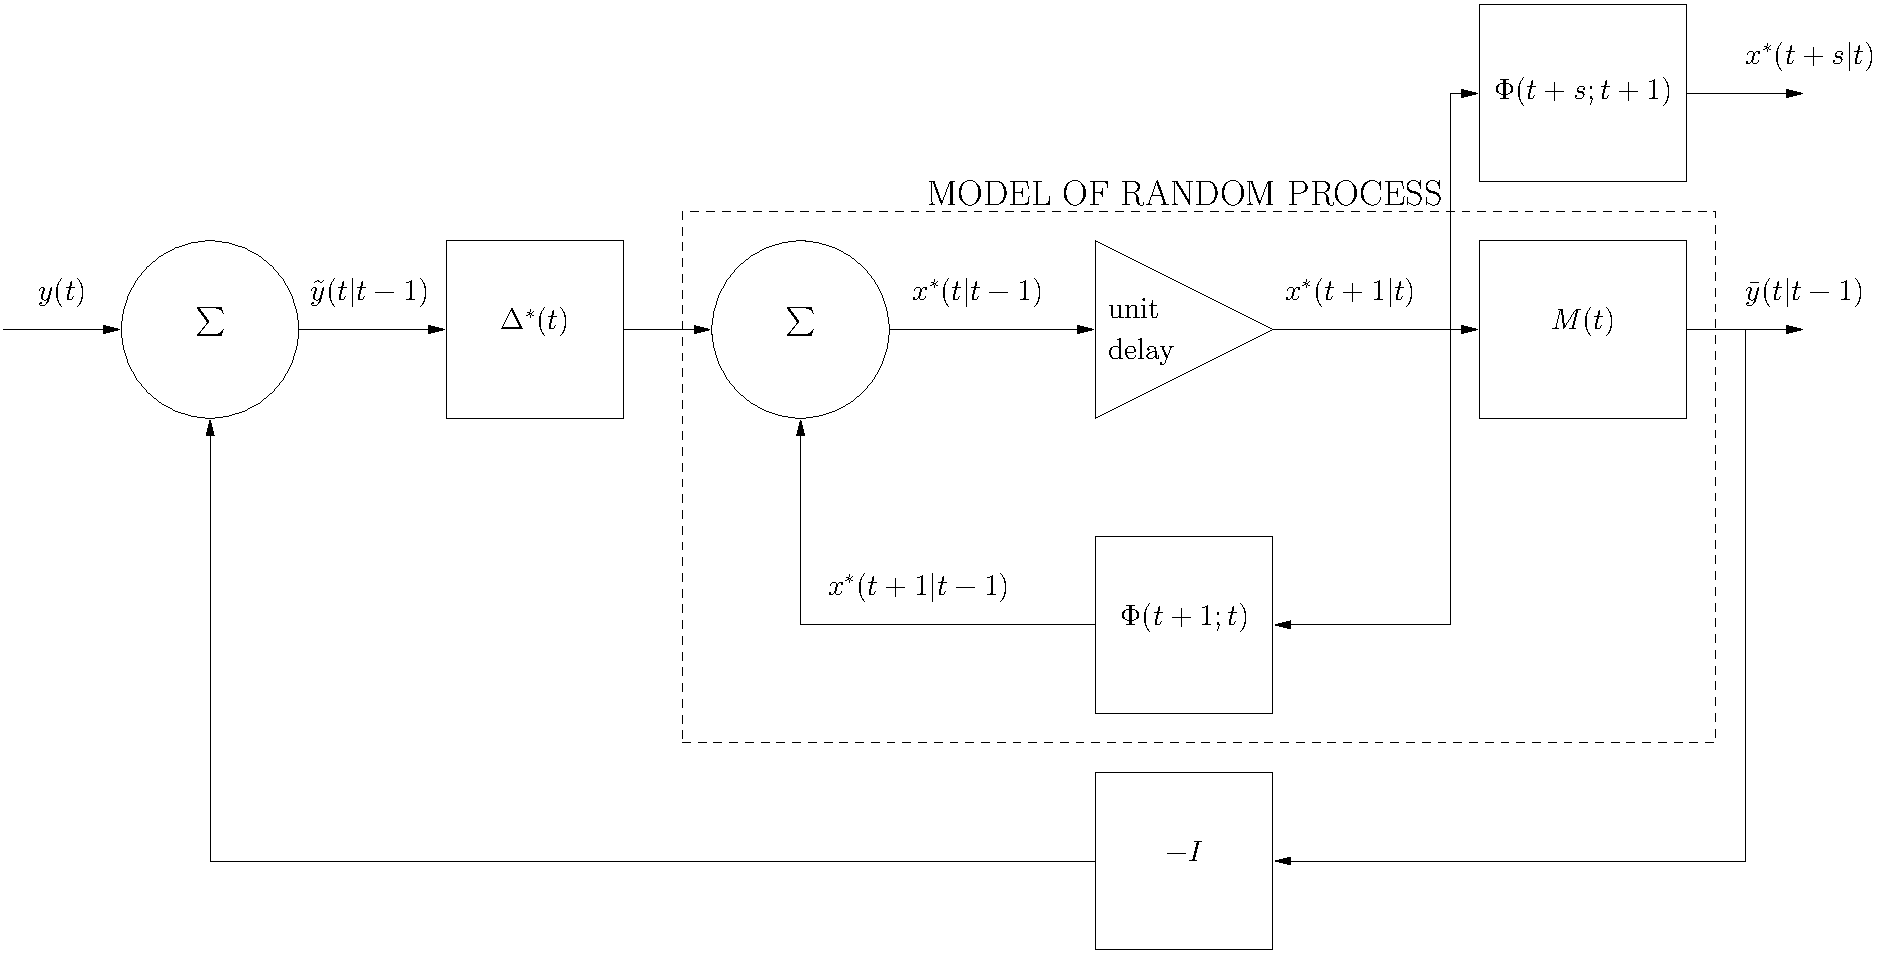
\includegraphics[width=0.5\paperwidth]{fig/fg3.pdf}
\caption{最优滤波器的矩阵框图}
\label{fg3}
\end{figure}
%TODO:

\section{对偶问题}
%TODO:
\begin{figure}[htbp]
\centering
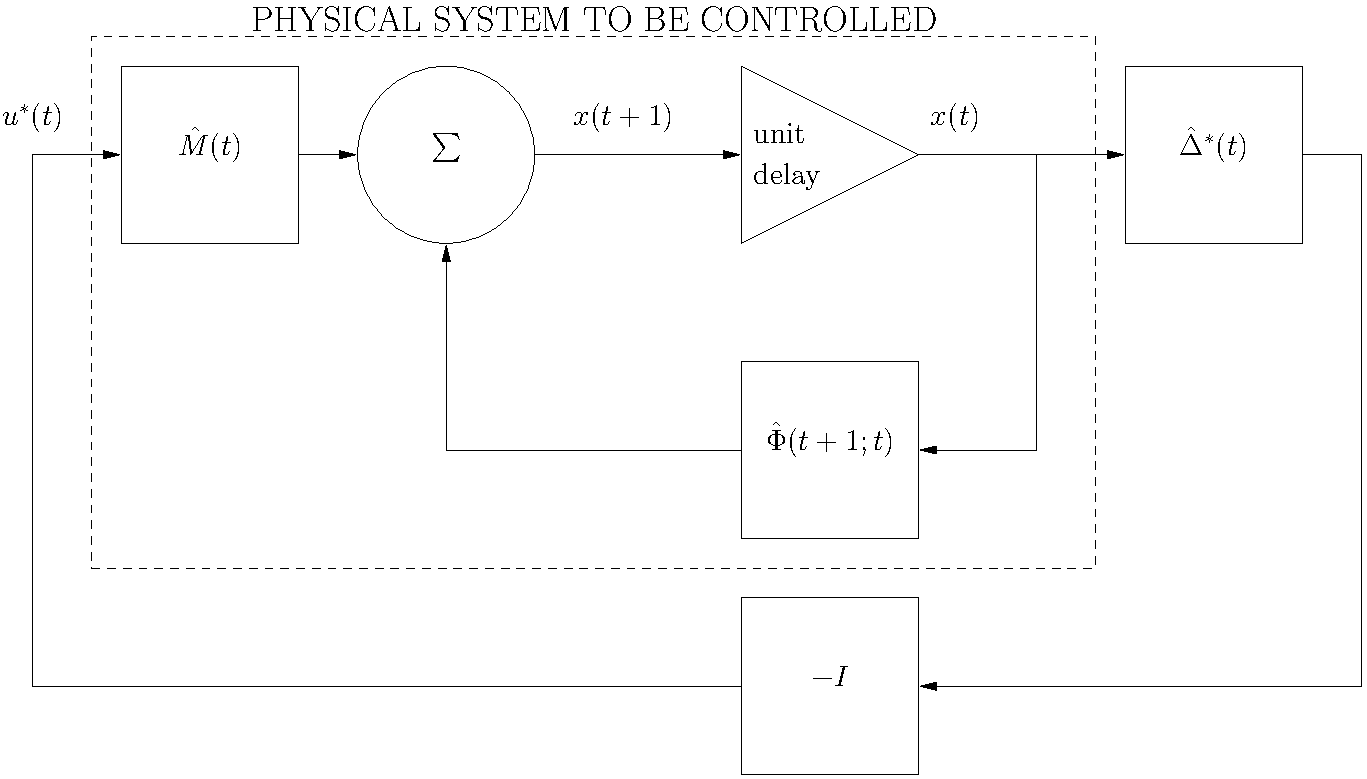
\includegraphics[width=0.5\paperwidth]{fig/fg4.pdf}
\caption{最优控制器的矩阵框图}
\label{fg4}
\end{figure}
%TODO:

\section{应用}
%TODO:
\section{结论}
本文从“状态”观点公式化并解决了Wiener问题。一方面,这引领我们找到一种常规的方法来处理问题(包括用其他方法将碰上困难的问题)。另一方面,这也证明Wiener问题与控制论中的其他问题紧密相连。为了探索这其中的联系,还需要更进一步的工作。

\begin{thebibliography}{0}
\bibitem{rf1} N. Wiener, ``The Extrapolation, Interpolation and Smoothing of Stationary Time Series,'' John Wiley \& Sons, Inc., New York, N. Y., 1949.
\bibitem{rf2} L. A. Zadeh and J. R. Ragazzini, ``An Extension of Wiener's Theory of Prediction,'' \textit{Journal of Applied Physics}, vol. 21, 1950. pp. 645-655.
\bibitem{rf3} H. W. Bode and C. E. Shannon, ``A Simplified Derivation of Linear Least-Squares Smoothing and Prediction Theory,'' \textit{Proceedings IRE}, vol. 38, 1950, pp. 417-425.
\bibitem{rf4} R. C. Booton, ``An Optimization Theory for Time-Varying Linear Systems with Nonstationary Statistical Inputs,'' \textit{Proceedings IRE}, vol. 40, 1952, pp. 977-981.
\bibitem{rf5} J. H. Laning and R. H. Battin, ``Random Processes in Automatic Control,'' McGraw-Hill Book Company, Inc., New York, N. Y., 1956.
\bibitem{rf6} W. H. Davenport, Jr., and W. L. Root, ``An Introduction to the Theory of Random Signals and Noise,'' McGraw-Hill Book Company, Inc., New York, N. Y., 1958.
\bibitem{rf7} S. Darlington, ``Linear Least-Squares Smoothing and Prediction, With Applications,'' \textit{Bell System Tech. Journal}, vol. 37, 1958, pp. 1221-1294.
\bibitem{rf8} G. Franklin, ``The Optimum Synthesis of Sampled-Data Systems'' Doctoral dissertation, Dept. of Elect. Engr., Columbia University, 1955.
\bibitem{rf9} A. B. Lees, ``Interpolation and Extrapolation of Sampled Data,'' \textit{Trans. IRE Prof. Group on Information Theory}, IT-2, 1956, pp. 173-175.
\bibitem{rf10} R. C. Davis, ``On the Theory of Prediction of Nonstationary Stochastic Processes,'' \textit{Journal of Applied Physics}, vol. 23, 1952, pp. 1047-1053.
\bibitem{rf11} M. Shibrot, ``Optimization of Time-Varying Linear Systems With Nonstationary Inputs,'' \textsc{Trans. ASME}, vol. 80, 1958, pp. 457-462.
\bibitem{rf12} M. Blum, ``Recursion Formulas for Growing Memory Digital Filters,'' \textit{Trans. IRE Prof. Group on Information Theory}, IT-4, 1958, pp. 24-30.
\bibitem{rf13} V. S. Pugachev, ``The Use of Canonical Expansions of Random Functions in Determining an Optimum Linear Systems,'' \textit{Automatics and Remote Control}(USSR), vol. 17, 1956, pp. 489-499; translation pp. 545-556.
\bibitem{rf14} V. V. Solodovnikov and A. M. Batkov, ``On the Theory of Self-Optimizing Systems (in German and Russian),'' Proc. Heidelberg Conference on Automatic Control, 1956, pp. 308-323.
\bibitem{rf15} J. L. Doob, ``Stochastic Processes,'' John Wiley \& Sons, Inc., New York, N. Y., 1955.
\bibitem{rf16} M. Lo\`eve, ``Probability Theory,'' Van Nostrand Company, Inc., New York, N. Y., 1955.
\bibitem{rf17} R. E. Bellman, I. Glicksberg, and O. A. Gross, ``Some Aspects of the Mathematical Theory of Control Processes,'' RAND Report R-313, 1958, 244 pp.
\bibitem{rf18} R. E. Kalman and R. W. Koepcke, ``Optimal Synthesis of Linear Sampling Control Systems Using Generalized Performance Indexes,'' \textsc{Trans. ASME}, vol. 80, 1958, pp. 1820-1826.
\bibitem{rf19} J. E. Bertram, ``Effect of Quantization in Sampled-Feedback Systems,'' \textit{Trans. AIEE}, vol. 77, II, 1958, pp. 177-182.
\bibitem{rf20} R. E. Kalman and J. E. Bertram, ``General Synthesis Procedure for Computer Control of Single and Multi-Loop Linear Systems,'' \textit{Trans. AIEE}, vol. 77, II, 1958, pp. 602-609.
\bibitem{rf21} C. W. Merriam, III, ``A Class of Optimum Control Systems,'' \textit{Journal of the Franklin Institute}, vol. 267, 1959, pp. 267-281.
\bibitem{rf22} R. E. Kalman and J. E. Bertram, ``A Unified Approach to the Theory of Sampling Systems,'' \textit{Journal of the Franklin Institute}, vol. 267, 1959, pp. 405-436.
\bibitem{rf23} R. E. Kalman and R. W. Koepcke, ``The Role of Digital Computers in the Dynamic Optimization of Chemical Reactors,'' Proc. Western Joint Computer Conference, 1959, pp. 107-116.
\bibitem{rf24} R. E. Kalman, ``Dynamic Optimization of Linear Control Systems, I. Theory,'' to appear.
\bibitem{rf25} S. Sherman, ``Non-Mean-Square Error Criteria,'' \textit{Trans. IRE Prof. Group on Information Theory}, IT-4, 1958, pp. 125-126.
\bibitem{rf26} V. S. Pugachev, ``On a Possible General Solution of the Problem of Determining Optimum Dynamic Systems,'' \textit{Automatics and Remote Control}(USSR), vol. 17, 1956,pp. 585-589.
\bibitem{rf27} G. C. Newton, Jr., L. A. Gould, and J. F. Kaiser, ``Analytical Design of Linear Feedback Controls,'' John Wiley \& Sons, Inc., New Youk, N. Y., 1957.
\bibitem{rf28} O. J. M. Smith, ``Feedback Control Systems,'' McGraw-Hill Book Company, Inc., New York, N. Y., 1958.
\bibitem{rf29} R. E. Kalman, ``On the General Theory of Control Systems,'' Proceedings First International Conference on Automatic Control, Moscow, USSR, 1960.
\end{thebibliography}

\appendix
\section{随机过程:基本概念}
为方便读者,我们在此对有关概率论以及随机过程的一些基本定义以及事实进行回顾。一切都用尽可能简明的方式展现;如需深入或延伸,可查阅Laning与Battin或Doob的工作。

\emph{随机变量}是取值依赖于偶然性事件之结果的函数。随机变量的\emph{值}可以是任意方便的数学量;实数或复数,矢量,等等。为了简明,我们在此将仅考虑实值随机变量,但这并非现实的约束。记随机变量为$x,y,\dotsc$, 并记其值为$\xi,\eta,\dotsc$. 随机变量的和、积、函数仍然是随机变量。

随机变量$x$可通过说明其小于或等于某个常数$\xi$的概率来显式的定义。可以用符号表示为
\begin{equation}
Pr(x\le\xi)=F_x(\xi)\text{;}F_x(-\infty)=0\text{,}F_x(+\infty)=1
\end{equation}
$F_x(\xi)$称为随机变量$x$的概率分布函数。当$F_x(\xi)$对$\xi$可导时$f_x(\xi)=\frac{dF_x(\xi)}{d\xi}$称为$x$的概率密度函数。

随机变量$x$的任意非随机函数$g(x)$的\emph{期望值}(\emph{数学期望、统计平均、系综平均、平均值}都是常见的同义词)定义为
\begin{equation}
\label{eq40}
Eg(x)=E[g(x)]=\int_{-\infty}^{\infty}g(\xi)dF_x(\xi)=\int_{-\infty}^{\infty}g(\xi)f_x(\xi)d\xi
\end{equation}
正如上文指出的,通常为了方便将会省略$E$后面的括号。随机变量(有限的或无限的)的序列
\begin{equation}
\label{eq41}
\{x(t)\}=\dotsc,x(-1),x(0),x(1),\dotsc
\end{equation}
叫做\emph{离散}(或\emph{离散参数})\emph{随机}(或\emph{概率性},此处原文为\emph{stochastic})\emph{过程}。式\ref{eq41}表示的随机过程的一组特定的观测值
\begin{equation*}
\dotsc,\xi(-1),\xi(0),\xi(1),\dotsc
\end{equation*}
称为该过程的\emph{实现}(或\emph{抽样函数})。直觉上,随机过程是一组编排好索引从而有了时间概念的随机变量。

称随机过程是\emph{不相关的},如果
\begin{equation*}
Ex(t)x(s)=Ex(t)Ex(s) \text{  (} t \ne s \text{)}
\end{equation*}
如果,更进一步的,
\begin{equation*}
Ex(t)x(s)=0 \text{  (} t \ne s \text{)}
\end{equation*}
则该随机过程是\emph{正交的}。将$x(t)$替换为$x'(t)=x(t)-Ex(t)$则任意不相关的随机过程都可以变成正交的随机过程,因为
\begin{equation*}
Ex'(t)x'(s)=E[x(t)-Ex(t)]\cdot[x(s)-Ex(s)]=Ex(t)x(s)-Ex(t)Ex(s)=0
\end{equation*}
记住这个实用的结论,如果某随机过程是正交的,那么
\begin{equation*}
E[x(t_1)+x(t_2)+\dotsc]^2=Ex^2(t_1)+Ex^2(t_2)+\dotsc \text{  (}t_1 \ne t_2 \ne \dotsc \text{)}
\end{equation*}
如果$\mathbf{x}$是以$x_1,\dotsc,x_n$(当然也是随机变量)为分量的矢量值随机变量,矩阵
\begin{equation}
\label{eq42}
[E(x_i-Ex_i)(x_j-Ex_j)]=E(\mathbf{x}-E\mathbf{x})(\mathbf{x'}-E\mathbf{x'})=\mathrm{cov}\text{ }\mathbf{x}
\end{equation}
称为$\mathbf{x}$的\emph{协方差矩阵}。

随机过程可以通过说明任意有限数量的如下类型的事例同时发生的概率来显式的明确说明
\begin{multline}
\label{eq43}
x(t_1) \le \xi_1,\dotsc,x(t_n) \le \xi_n \text{;}\text{(}t_1 \ne \dotsc \ne t_n \text{), i.e., }\\
Pr[(x(t_1) \le \xi_1, \dotsc, x(t_n) \le \xi_n)]=F_{x(t_1),\dotsc,x(t_n)}(\xi_1,\dotsc,\xi_n)
\end{multline}
其中$F_{x(t_1),\dotsc,x(t_n)}$叫做随机变量$x(t_1), \dotsc, x(t_n)$的\emph{联合概率分布函数}。这样,\emph{联合概率密度函数}即为
\begin{equation*}
f_{x(t_1),\dotsc,x(t_n)}(\xi_1,\dotsc,\xi_n)=\frac{\partial^n F_{x(t_1),\dotsc,x(t_n)}}{\partial\xi_1,\dotsc,\partial\xi_n}
\end{equation*}
,假如需要的导数存在。$n$个随机变量的任意非随机函数的期望值$Eg[x(t_1),\dotsc,x(t_n)]$由类似式\ref{eq40}的$n$重积分定义。

如果对于任意有限个$t_1 \ne \dotsc \ne t_n$式\ref{eq43}等于一阶分布的积
\begin{equation*}
Pr[x(t_1) \le \xi_1] \dotsc Pr[x(t_n) \le \xi_n]
\end{equation*}
则该随机过程是\emph{独立的}。如果一组随机变量是独立的,显然它们也是不相关的。但是一般来说,反过来则并不成立。对于多于两个随机变量的一个集合,任意两个互相独立并不足以使整个集合是独立的。

给定随机变量$x(t_1),\dotsc,x(t_n)$出现的实际值$\xi_1,\dotsc,\xi_n$来考虑随机变量$x(t_{n+1}$的概率分布常常是人们关注的。记此分布为
\begin{multline}
\label{eq44}
Pr[x(t_{n+1} \le \xi_{n+1} \vert x(t_1)=\xi_1,\dotsc,x(t_n)=\xi_n]\\
=\frac{\int^{\xi_{n+1}}_{-\infty}f_{x(t_1),\dotsc,x(t_{n+1})}(\xi_1,\dotsc,\xi_{n+1})d\xi_{n+1}}{f_{x(t_1),\dotsc,x(t_n)}(\xi_1,\dotsc,\xi_n)}
\end{multline}
并称之为给定$x(t_1),\dotsc,x(t_n)$的$x(t_{n+1}$的\emph{条件概率分布函数}。条件期望
\begin{equation*}
E\{g[x(t_{n+1})] \vert x(t_1),\dotsc,x(t_n)\}
\end{equation*}
的定义类似式\ref{eq40}. 条件期望是一个随机变量;它服从
\begin{equation*}
E[E\{g[x(t_{n+1})] \vert x(t_1),\dotsc,x(t_n)\}]=E\{g[x(t_{n+1})]\}
\end{equation*}

在本文所关注的所有情况中,如式\ref{eq40}或者式\ref{eq44}的积分并不需要显式的计算出来,只有期望值的\emph{概念}是需要的。

随机变量$x$是\emph{高斯的}(或者\emph{正态分布的}),如果
\begin{equation*}
f_x(\xi)=\frac{1}{[2 \pi E(x-Ex)^2]^{\frac{1}{2}}}exp[-\frac{1}{2}\frac{(\xi-Ex)^2}{E(x-Ex)^2}]
\end{equation*}
亦即人们熟知的钟状曲线。类似的,随机矢量$\mathbf{x}$是\emph{高斯的},如果
\begin{equation*}
f_{\mathbf{x}}(\mathbf{\xi})=\frac{1}{(2\pi)^{\frac{n}{2}}(\mathrm{det}\text{ }\mathbf{C})^{\frac{1}{2}}}exp[-\frac{1}{2}(\mathbf{\xi}-E\mathbf{x})'\mathbf{C}^{-1}(\mathbf{\xi}-E\mathbf{x})]
\end{equation*}
其中$\mathbf{C}^{-1}$是$\mathbf{x}$协方差矩阵(式\ref{eq42})的逆。类似的可以定义\emph{高斯随机过程}。

高斯随机变量与随机过程的重要性大体上是由于下列事实:
\begin{theorem}
\label{th5}
\begin{itemize}
\item[A] 高斯随机过程的线性函数(因而有条件期望)是高斯随机变量。
\item[B] 正交高斯随机变量是独立的。
\item[C] 给定任意均值为$Ex(t)$, 协方差为$Ex(t)x(s)$的随机过程,存在唯一的高斯随机过程具备同样的均值与协方差。
\end{itemize}
\end{theorem}
\end{document}
